\documentclass[3p]{elsarticle}

% APS journals: PRL and PRF
% Note: All AIP and APS journals use the revtex package; both PRL and PRF are APS.
%\documentclass[preprint, superscriptaddress, notitlepage]{revtex4-1}

% Physica D is elsevier 
%\documentclass[review]{elsarticle}

%\documentclass{jfm}
% NOTE: jfm documentclass needed for \upi
%---------------------------------------------------%
% Packages from JFM 2020
%\usepackage[top=1.2in,bottom=1.2in,left=1in, right=1in]{geometry}
\usepackage{amsfonts, amssymb, array}
\usepackage[fleqn,reqno]{amsmath}
\usepackage{graphics, graphicx, subfigure}
% Replaced subcaption with subfigure
\usepackage{todonotes, comment, soul, float}
%---------------------------------------------------%

%^^^^^^^^^^^^^^^^^^^^^^^^^^^^^^^^^^^^^^^^^^^^^^^^^^^^^^^^^^^^%
% COMMANDS
% Basic editing
\newcommand{\vsp}[1]{\vspace{#1 pc} \noindent}
\newcommand{\np}{\newpage \noindent}
\newcommand{\tocite}{ {\color{blue}(to cite)} }
\newcommand{\nick}[1]{ {\color{red} #1} }
% For real and imaginary, could use \Re or \Im, or \mathcal{R}, or \text{Re}
\newcommand{\Real}{\Re}
\newcommand{\Imag}{\Im}

%---------------------------------------------------%
% From JFM 2020
\newcommand{\bd}{{\partial}}
\newcommand{\bigO}{{\mathcal{O}}}
\newcommand{\cc}{{\mathbf{c}}}
\newcommand{\CC}{{\mathbb{C}}}
\newcommand{\DD}{{\mathcal{D}}}
\newcommand{\DDD}{{\boldsymbol{\mathcal D}}}
\newcommand{\eeta}{{\boldsymbol\eta}}
\newcommand{\ff}{{\mathbf{f}}}
\newcommand{\grad}{{\nabla}}
\newcommand{\II}{{\mathbf{I}}}
\newcommand{\iin}{\mathrm{in}}
\newcommand{\llambda}{{\boldsymbol\lambda}}
\newcommand{\nn}{{\mathbf{n}}}
\newcommand{\NN}{{\mathcal{N}}}
\newcommand{\out}{\mathrm{out}}
\newcommand{\rr}{{\mathbf{r}}}
\renewcommand{\Re}{{\operatorname{Re}}}
\renewcommand{\Im}{{\operatorname{Im}}}
\newcommand{\RR}{{\mathbb{R}}}
\renewcommand{\ss}{{\mathbf{s}}}
\newcommand{\tar}{\mathrm{tar}}
\newcommand{\bary}{\mathrm{bary}}
\newcommand{\trap}{\mathrm{trap}}
\newcommand{\uu}{{\mathbf{u}}}
\newcommand{\UU}{{\mathbf{U}}}
\newcommand{\vv}{{\mathbf{v}}}
\newcommand{\xx}{{\mathbf{x}}}
\newcommand{\xxi}{{\boldsymbol{\xi}}}
\newcommand{\yy}{{\mathbf{y}}}
\newcommand{\mcaption}[2]{\caption{\small \em #1}\label{#2}} 
\newcommand{\secref}[1]{\ref{#1}}
\def\gap{\hspace*{.2in}}
% Nick's below
\newcommand{\pderiv}[2]{\frac{\partial #1}{\partial #2}}
\newcommand{\ppd}[2]{\frac{\partial^2 #1}{{\partial #2}^2}}
\newcommand{\abs}[1]{\left| #1 \right|}
\newcommand{\Vn}{V_\nn}
\newcommand{\Vs}{V_\ss}
\newcommand{\CE}{C_E}
%---------------------------------------------------%

% From Nick's Latex Notes
\newcommand{\bvec}[1]{\mathbf{#1}}
%{\ensuremath{\boldsymbol{#1}}}
\newcommand {\bq} {\bvec{q}}
\newcommand{\mean}[1]{\left< #1 \right>}
\newcommand{\qavg}{\bar{q}}
\newcommand{\pavg}{\bar{p}}
\newcommand{\pup}{p_u}
\newcommand{\pdn}{p_d}
\newcommand{\stress}{{\boldsymbol \sigma}}
\newcommand{\FD}{\bvec{F}_d}
\newcommand{\ex}{ {\bvec{e}}_1}

% New
\newcommand{\anis}{\mathcal{A}}
\newcommand{\diag}{\mathop{\mathrm{diag}}}


%^^^^^^^^^^^^^^^^^^^^^^^^^^^^^^^^^^^^^^^^^^^^^^^^^^^^^^^^^^^^%
% TITLE AUTHORS ABSTRACT
\begin{document}
\title{How fluid-mechanical erosion creates anisotropic porous media}

% Maybe HOW fluid-mechanical erosion creates anisotropic porous media.
%\title{Fluid-mechanical erosion generates anisotropy in porous media}
%\title{Erosion leads to anisotropy in a porous medium}
%\title{The development of anisotropy in an eroding porous medium}


\author[Colgate]{Nicholas J.~Moore}

\author[FSU]{Jake Cherry}

\author[NJIT]{Shang-Huan Chiu}
%\affiliation{Department of Scientific Computing, Florida State University, Tallahassee, FL, 32306.}

\author[FSU]{Bryan D.~Quaife}
%\address{\FSU}

\address[Colgate]{Colgate University}
\address[FSU]{Florida State University}
\address[NJIT]{New Jersey Institute of Technology}

\begin{abstract}
Using a Cauchy integral formulation of the boundary integral equations, we simulate the erosion a porous medium comprised of $O(100)$ solid bodies embedded in a Stokes flow. The grains of the medium are resolved individually and erode under the action of surface shear stress. In particular, detailed changes in grain morphology are resolved, and these microscopic changes give rise to larger-scale features in the medium such as channelization. The Cauchy-integral formulation and associated quadrature formulas enable us to resolve configurations of tightly packed and nearly contacting bodies. We observe substantial anisotropy to develop over the course of erosion; that is, the configurations that result from erosion generally permit flow in the longitudinal direction more easily than in the transverse direction by a factor up to five.  \\
Tie it to alternate hypothesis in groundwater.
\end{abstract}
\maketitle

% Original ideas
%We numerically simulate the erosion of a porous medium due to an internally flowing fluid, with solid constituents of the medium eroding under the action of surface shear stress. 
%We numerically simulate the erosion of a porous medium due to an internally flowing fluid.  The solid constituents of the porous medium erode under the action of surface shear stress. As the particles disintegrate, they elongate in the direction of the flow, giving rise to anisotropic conductivity of the porous medium.

% dematerialize, disintegrate
% internal, permeating, intervening
%^^^^^^^^^^^^^^^^^^^^^^^^^^^^^^^^^^^^^^^^^^^^^^^^^^^^^^^^^^^^%


\section{Introduction}

Flow-induced erosion acts across a range of scales in the natural world, from massive geological structures sculpted by wind or water \cite{abrams2009growth, perkins2015amplification, mac2020ultra, sharma2022alcove, mac2022morphological}, to mesoscopic patterns formed by surface or internal flows \cite{berhanu2012shape, bertagni2021hydrodynamic}, and down to the granular constituents of porous media as they slowly disintegrate in groundwater flows \cite{zareei2022temporal}. The shape-flow feedback of erosion can imprint across all of these scales, affecting both large-scale features and small-scale ones, such as the microstructure of porous materials.
The porous media encountered in nature, for example, typically exhibit material {\em anisotropy} in that they permit seepage flow in certain directions more easily than in others. Typical materials are more permeable to flow in the longitudinal (or horizontal) direction than transversely by a factor of 5-20 \cite{bear1988dynamics, anderson2015applied}. Most commonly, this material anisotropy is attributed to the sedimentation process, in which, due to the fluid-structure interaction, non-spherical particles tend to settle with their long axis parallel to the plan of deposition \cite{bear1988dynamics}. Controlled experiments, however, have not been performed to test this hypothesis, and other mechanisms may be at work. Here, we use highly-accurate numerical simulations to examine an alternative, and possibly complementary, mechanism: namely, that the flow-induced erosion of the medium's solid constituents contributes to its overall anisotropy.

Our method merges highly-efficient and highly-accurate boundary-integral equation (BIE) methods with stable interface evolution methods to simulate the erosion of dense suspensions of solid bodies in the Stokes regime of groundwater flow \cite{quaife2018boundary}. Originally inspired by related work in the high-Reynolds-number regime \cite{Ristroph2012, Moore2013, Huang2015, MooreCPAM2017}, our method is documented, validated, benchmarked in \cite{quaife2018boundary}, and can simulate the erosion of $O(100)$ solid bodies. The more recent Cauchy reformulation of the BIE and the associated  quadrature formulas allow us to resolve points of near contact between bodies, thus enabling high-fidelity simulation of dense suspensions of erodable bodies \cite{chiu2020viscous}.

\vsp{5}


Figure \ref{FigVortVel} shows an example illustration of 80 eroding bodies

%Maybe cite: \cite{Rycroft2016}
% Cite paper by Ladd "Wormhole formation in dissolving fractures"

%^^^^^^^^^^^^^^^^^^^^^^^^^^^^^^%
\begin{figure*}[] \centering
        \subfigure[ Vorticity field]{ \label{FigVort}
            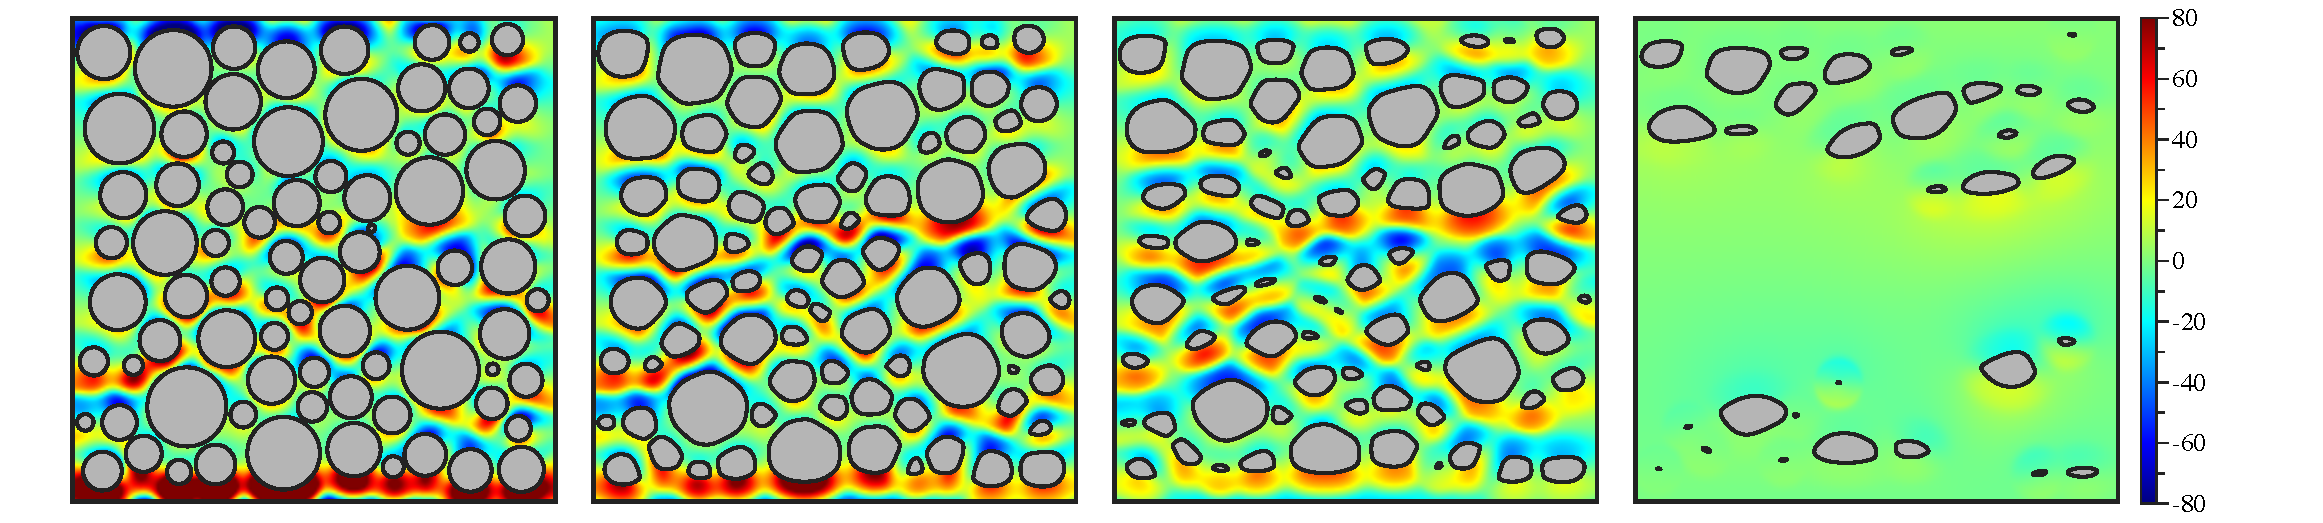
\includegraphics[width=0.9 \textwidth]{figs/80circ8vort.pdf} } \\
        \subfigure[ Velocity magnitude]{ \label{FigVel}
            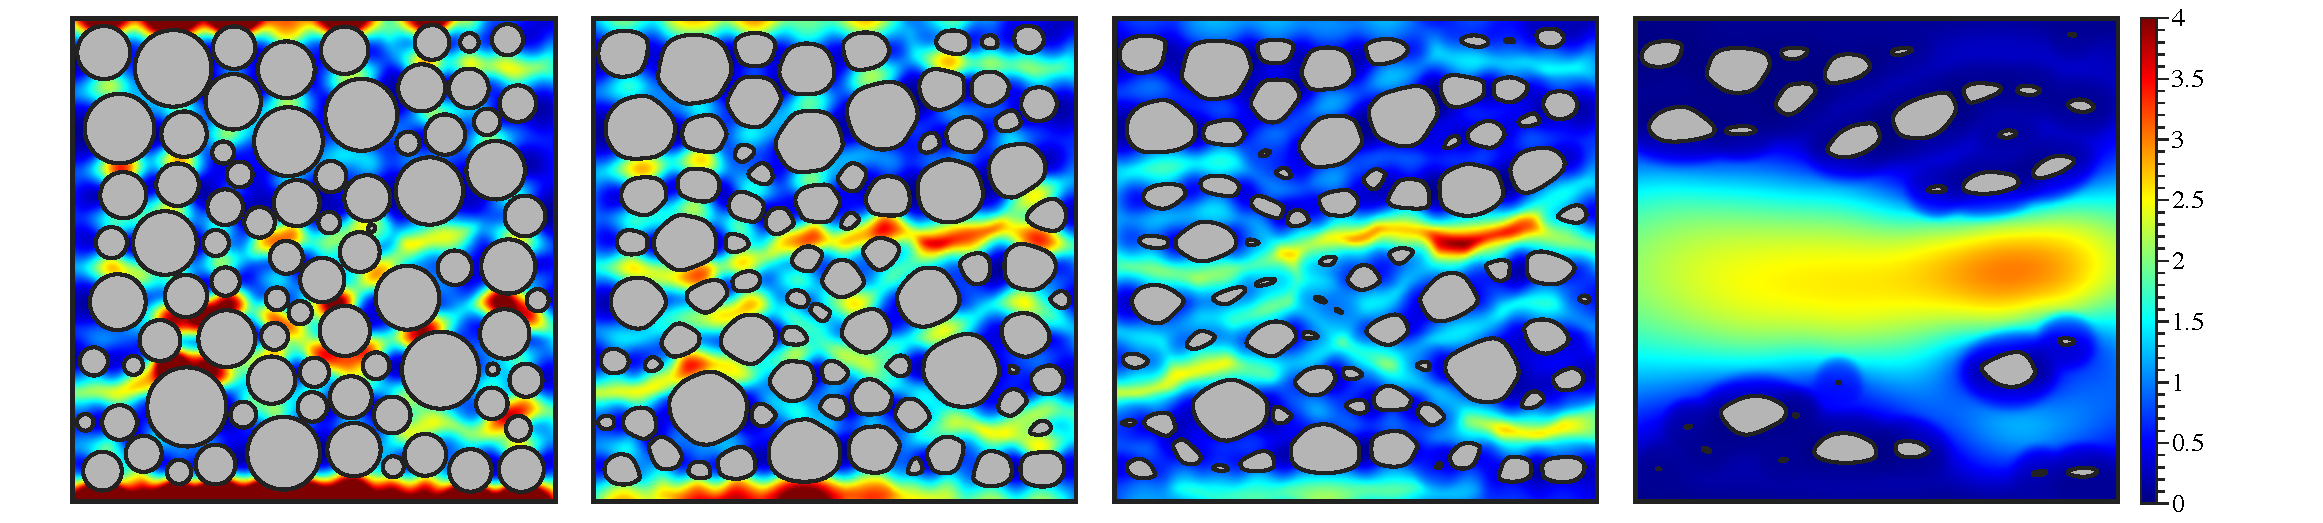
\includegraphics[width=0.9 \textwidth]{figs/80circ8vel.pdf} }
   \caption{80 eroding bodies}
   \label{FigVortVel}
\end{figure*}
%^^^^^^^^^^^^^^^^^^^^^^^^^^^^^^%
% Data from 80circ8

\begin{comment}
%^^^^^^^^^^^^^^^^^^^^^^^^^^^^^^%
\begin{figure*}%[htbp]
\centering \label{fig1}
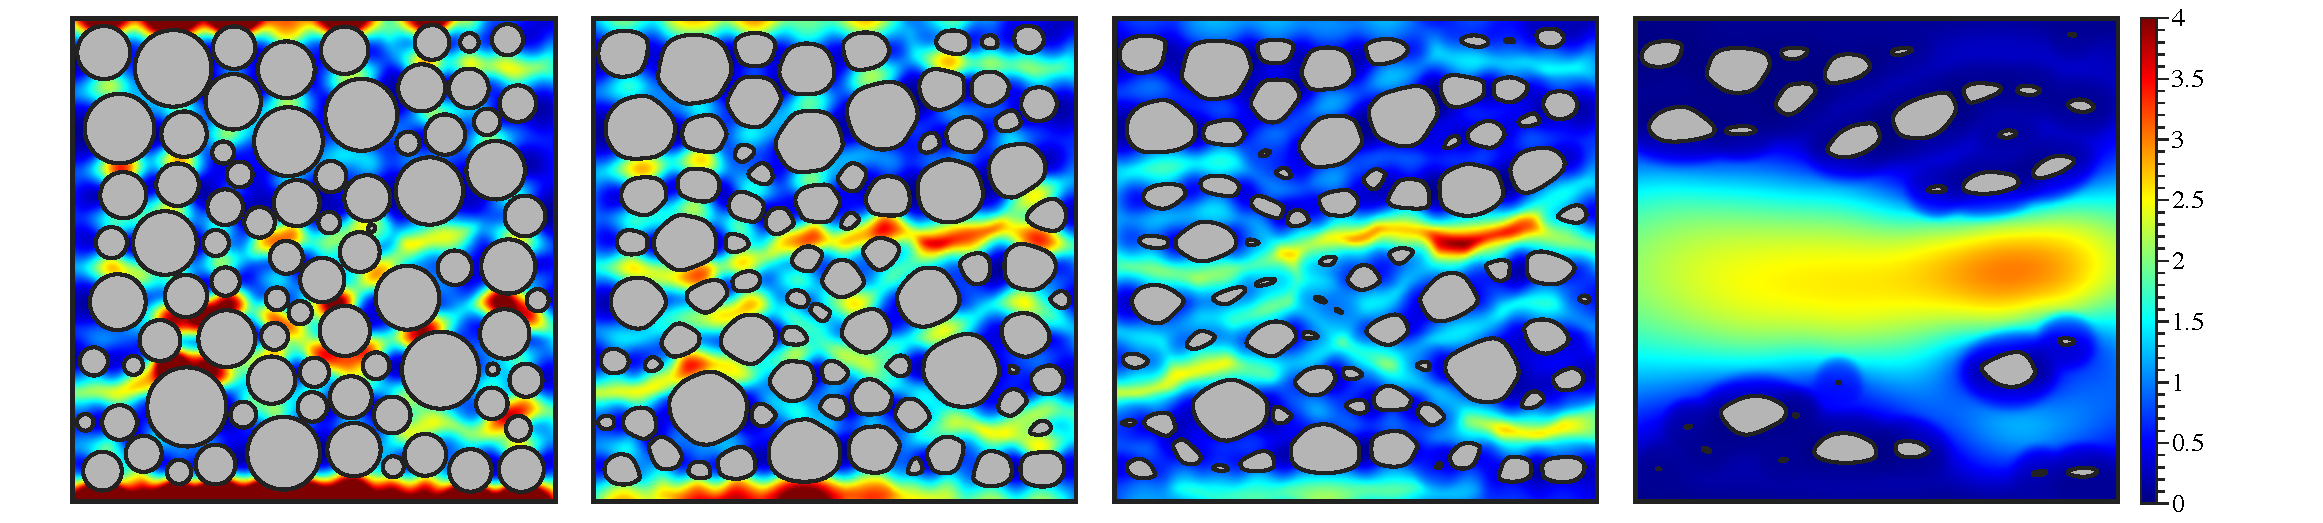
\includegraphics[width = 0.9 \textwidth]{./figs/80circ8vel.pdf}
\caption{caption}
\end{figure*}
 %^^^^^^^^^^^^^^^^^^^^^^^^^^^^^^%
\end{comment}



%-----------------------------------------------------------------------------------------------%
\section{Governing Equations}
\label{sec:formulation}
%-----------------------------------------------------------------------------------------------%

Consider an incompressible, Stokes flow inside a domain $\Omega$ containing $M$ erodable bodies. We take the outer boundary $\Gamma$ to be a slightly smoothed version of the boundary of $[-3,3] \times [-1,1]$. The fluid flow is primarily from left to right, so that the inlet and outlet are located at approximately $x=-3$ and $+3$ respectively (the actual locations are slightly curved versions of these vertical lines due to domain smoothing). The erodable bodies, with boundaries $\gamma_\ell$, $\ell = 1,\ldots,M$, all sit inside of the central region $[-1,1] \times [-1,1]$. The boundary of the fluid domain is thus $\bd \Omega = \Gamma \cup \gamma_1 \cup \cdots \cup \gamma_M$. 
The empty space to the left and right of $[-1,1] \times [-1,1]$ serve as buffer regions to allow the flow profile imposed at the inlet and outlet to gradually adjust to the presence of the bodies. The equations governing the velocity $\uu$ and pressure $p$ of the fluid consist of the incompressible, Stokes equations coupled to boundary conditions:
\begin{equation}
\label{eqn:StokesEq}
  \begin{split}
    \mu \Delta \uu = \grad p, &\hspace{20pt} \xx \in \Omega, \gap 
      &&\mbox{\em conservation of momentum}, \\
    \grad \cdot \uu = 0, &\hspace{20pt} \xx \in \Omega, \gap 
      &&\mbox{\em conservation of mass}, \\
    \uu = \mathbf{0}, &\hspace{20pt} \xx \in \gamma, \gap 
      &&\mbox{\em no slip on the erodable bodies}, \\
    \uu = \UU, &\hspace{20pt} \xx \in \Gamma, \gap 
      &&\mbox{\em outer wall velocity}.
  \end{split}
\end{equation}
Above, $\UU$ represents the fluid velocity imposed along the outer boundary $\Gamma$, in particular at the inlet and outlet, as well as along the top and bottom walls. In this work, we impose a {\em uniform} flow profile along $\Gamma$, i.e.~$\UU = (U,0)$, although other choices are possible, for example a Poiseuille profile as employed in previous work \cite{quaife2018boundary, chiu2020viscous}. The advantages of the uniform profile are: (1) it will simplify the calculation of porous-medium properties, such as permeability and anisotropy, that will be described later; and (2), it may more realistically model the flow impinging upon a porous medium. We will allow the imposed flow speed to change with time $U = U(t)$ to enforce, for example, a desired pressure drop across the flow cell. To nondimensionalize the above system, we set the fluid viscosity to unity, $\mu = 1$.

The embedded bodies may erode in response to the shear stresses induced by the intervening fluid flow. Erosion typically occurs over much longer timescales than does the fluid flow, permitting a {\em quasi-steady} approximation. In this approximation, the configuration of bodies is held fixed in order to compute the {\em steady} Stokes flow determined by \eqref{eqn:StokesEq}, and then this flow field determines the stresses acting to erode each body. We employ an erosion law in which the local rate of material loss is linearly proportional to the magnitude of the shear stress $\tau$ acting on the surface (CITE previous erosion work). The material loss gives rise to an inward velocity of the solid surface, $\Vn$, pointing in the direction normal to the surface. The erosion law is thus expressed as
\begin{align}
\Vn = \CE \, \abs{\tau}, 
	&\hspace{20pt} \xx \in \gamma, &&\mbox{\em erosion model}, \\
\tau = -\mu \left( ( \nabla \uu + \nabla \uu^T) \nn \right) \cdot \ss
	&\hspace{20pt} \xx \in \gamma, &&\mbox{\em shear stress}.
  \label{eqn:shearStress}
\end{align}
where $\nn$ is a unit normal vector pointing into each body, $\ss$ is
a unit tangent vector pointing in the counterclockwise direction, and $\CE$ is a material-dependent erosion constant.

% SNIPPETS 
%The strength of $\UU$ is adjusted at each time step to achieve a constant pressure drop across the channel, motivated by the geological situation of a porous medium connecting two regions of  fixed hydraulic heads.

%to transition to the more complex flow intervening between the bodies.


%-----------------------------------------------------------------------------------------------%
\section{Boundary Integral Equation and Cauchy Integral Formulation}
\label{sec:DLP}
%-----------------------------------------------------------------------------------------------%
To accurately and efficiently solve the Stokes
  equations~\eqref{eqn:StokesEq}, we reformulate the system as a
  boundary integral equation (BIE). A BIE formulation has the advantage
  that all the unknowns are on the one-dimensional boundary of the
  domain. Therefore, only the boundary of the complex geometry must be
  discretized which we do with a spectrally accurate Fourier basis.
  Applying the same approach as our previous
  works~\citep{quaife2018boundary, chiu2020viscous}, we represent the
  velocity as the sum of a double-layer potential and a combination of
  Stokeslets and rotlets~\cite{pow-mir1987}
\begin{align}
  \uu(\xx) = \DDD[\eeta](\xx) + \sum_{\ell=1}^{M}\left(
    S[\llambda_\ell](\xx) + R[\xi_\ell](\xx)\right), 
    \quad \xx \in \Omega,
  \label{eqn:velocity}
\end{align}
where 
\begin{align}
  \DDD[\eeta](\xx) = \frac{1}{\pi}\int_{\bd\Omega} 
  \frac{\rr \cdot \nn}{\rho^2} \frac{\rr \otimes \rr}{\rho^2}
  \eeta(\yy) \, ds_\yy.
  \label{eqn:velocityDLP}
\end{align}
Note that $\bd\Omega$ includes both the eroding bodies and the outer
boundary. The Stokeslet and the rotlets are
\begin{align}
  S[\lambda_\ell](\xx) = \frac{1}{4\pi} \left(-\log \rho_\ell +
  \frac{\rr_\ell \otimes \rr_\ell}{\rho_\ell^2} \right) \llambda_\ell,
  \quad
  R[\xi_\ell](\xx) = \frac{\rr_\ell^\perp}{\rho_\ell^2}\xi_\ell,
\end{align}
respectively, where $\rr_\ell = \xx - \cc_\ell$, $\rho_\ell =
\|\rr_\ell\|$, and $\cc_\ell$ is a point inside body $\ell$. If the
density function, Stokeslets, and rotlets satisfy the second-kind
boundary integral equation
\begin{subequations}
  \label{eqn:FredBIE}
  \begin{alignat}{3}
    \UU(\xx) &= -\frac{1}{2}\eeta(\xx) + \DDD[\eeta](\xx) + 
      \sum_{\ell=1}^{M}\left(S[\llambda_\ell](\xx) + R[\xi_\ell](\xx)\right), 
      \quad &&\xx \in \Gamma, \\
    \mathbf{0} &= -\frac{1}{2}\eeta(\xx) + \DDD[\eeta](\xx) + 
      \sum_{\ell=1}^{M}\left(S[\llambda_\ell](\xx) + R[\xi_\ell](\xx)\right), 
      &&\xx \in \gamma_\ell, \: \ell = 1,\ldots,M, \\
    \llambda_\ell &= \int_{\gamma_\ell} \eeta(\yy) \, ds_\yy, 
      &&\ell = 1,\ldots,M, \\
    \xi_\ell &= \int_{\gamma_\ell} (\yy - \cc_\ell)^\perp \cdot 
      \eeta(\yy) \, ds_\yy, &&\ell = 1,\ldots,M,
  \end{alignat}
\end{subequations}
then the representation~\eqref{eqn:velocity} satisfies the Stokes
equations with the required boundary conditions~\eqref{eqn:StokesEq}. We
solve~\eqref{eqn:FredBIE} by discretizing $\gamma_\ell$ and $\Gamma$ at
equispaced collocation points, and then replacing the integrals with
quadrature rules. This results in a linear system with a
mesh-independent condition number, and it is solved iteratively with
GMRES.

Instead of evaluating the Stokes double-layer
potential~\eqref{eqn:velocityDLP} as a contour integral in $\RR^2$, we
convert the integral to a sum of contour integrals around Jordan curves
in $\CC$. We identify $\xx = (x_1,x_2)$ with $x = x_1 + ix_x$, and use
similar notation for $\yy$, $\nn$, and $\eeta$. We also interpret
$\gamma$, the boundary of the $i^{th}$ grain or the bounding box
$\Gamma$, as a Jordan curve in $\CC$. We introduce the functions
\begin{align}
  \tau_1(y) = \eta(y) \overline{n(y)} \Re(n(y)), \quad 
  \tau_2(y) = \eta(y) \overline{n(y)} \Im(n(y)).
\end{align}
We then define the five Cauchy integrals
\begin{align}
  v_1(x) &= \frac{1}{2\pi i} \int_{\gamma} \frac{Re(\eta(y))}{x-y} \,dy, 
  \quad
  v_2(x) = \frac{1}{2\pi i} \int_{\gamma} \frac{Im(\eta(y))}{x-y} \, dy, 
  \quad
  v_3(x) = \frac{1}{2\pi i} \int_{\gamma} \frac{Re(\overline{y}\eta(y))}{x-y} \, dy, \\
  v_4(x) &= \frac{1}{2\pi i} \int_{\gamma} \frac{\tau_1(y)}{x-y} \, dy,
  \quad
  v_5(x) = \frac{1}{2\pi i} \int_{\gamma} \frac{\tau_2(y)}{x-y} \, dy.
\end{align}
Then, the first and second components of the Stokes double-layer
potential are
\begin{subequations}
  \begin{align}
    u_1(x) &= -\Re(x)\Re(v_1'(x)) - \Im(x)\Re(v_2'(x)) + 
             \Re(v_3'(x)) + \Re(v_4(x)) \\
    u_2(x) &= +\Re(x)\Im(v_1'(x)) + \Im(x)\Im(v_2'(x)) - 
             \Im(v_3'(x)) + \Re(v_5(x)),
  \end{align}
  \label{eqn:velocityCauchy}
\end{subequations}
respectively. The components of the deformation tensor are
\begin{subequations}
  \begin{align}
    \pderiv{u_1}{x_1} &= -\Re(v'_1(x)) + \Re(v''_3(x)) + \Re(v'_4(x))
                         -\Re(x)\Re(v''_1(x)) - \Im(x)\Re(v''_2(x)) \\
    \pderiv{u_1}{x_2} &= -\Re(v'_2(x)) - \Im(v''_3(x)) - \Im(v'_4(x))
                         +\Re(x)\Im(v''_1(x)) + \Im(x)\Im(v''_2(x)) \\
    \pderiv{u_2}{x_1} &= +\Im(v'_1(x)) - \Im(v''_3(x)) + \Re(v'_5(x))
                         +\Re(x)\Im(v''_1(x)) + \Im(x)\Im(v''_2(x)) \\
    \pderiv{u_2}{x_2} &= +\Im(v'_2(x)) - \Re(v''_3(x)) - \Im(v'_5(x))
                         +\Re(x)\Re(v''_1(x)) + \Im(x)\Re(v''_2(x)) 
  \end{align}
  \label{eqn:deformationCauchy}
\end{subequations}
Having the deformation tensor at hand, the vorticity can be shown to
satisfy
\begin{align}
  \omega(x) = \pderiv{u_2}{x_1} - \pderiv{u_1}{x_2} = 
     \Im(v_1'(x)) + \Re(v_2'(x)) + \Re(v_5'(x)) + \Im(v_4'(x)).
  \label{eqn:vorticityCauchy}
\end{align}
We note that the deformation tensor requires second-order derivatives of
Cauchy integrals, while the vorticity only requires first-order
derivatives.

%%%%%%%%%%%%%%%%%%%%%%%%%%%%%%%%%%%%%%%%%%%%%%%%%%%%%%%%%%%%%%%%%%%%%%%
\subsection{Quadrature for Cauchy integrals}
The accuracy of our method is determined by the accuracy of the
quadrature rule applied to equation~\eqref{eqn:FredBIE}. Since we have
written the Stokes double-layer potential
velocity~\eqref{eqn:velocityCauchy}, deformation
tensor~\eqref{eqn:deformationCauchy}, and
vorticity~\eqref{eqn:vorticityCauchy} as a sum of Cauchy integrals and
their derivatives, the accuracy of the method depends on the accuracy of
computing a general Cauchy integral
\begin{align}
  v(x) = \frac{1}{2\pi i} \int_{\gamma} \frac{\eta(y)}{x-y} \, dy.
  \label{eqn:cauchy1}
\end{align}
Here we describe a quadrature formulae that was first used to
approximate analytic functions~\cite{ioa-pap-per1991}, and then extended
to Stokes layer potentials~\cite{bar-wu-vee2015}. The quadrature method
requires the boundary data of the analytic function~\eqref{eqn:cauchy1}
which satisfies the Sokhotski-Plemelj jump relation
\begin{align}
  v^{-}(x_0) = \lim_{\substack{x \rightarrow x_0 \\ x \in \Omega}} \int_{\gamma}
    \frac{\eta(y)}{x-y}\, dy = -\frac{1}{2}\eta(x_0) - 
    \frac{1}{2\pi i} \int_{\gamma} \frac{\eta(y)}{x-y} \, dy,
    \quad x_0 \in \gamma,
    \label{eqn:SP}
\end{align}
where the last integral is interpreted in the principal value sense.
Here we are assuming that $\Omega$ is the bounded region interior to
$\gamma$. Once $v^{-}$ is calculated, $v(x)$ and its derivatives can be
determined by its boundary data alone using the Cauchy Integral Theorem
\begin{subequations}
  \label{eqn:cauchy}
  \begin{alignat}{3}
  \label{eqn:cauchyv}
  v(x) &= \frac{1}{2\pi i}\int_{\gamma} 
    \frac{v^{-}(y)}{y-x} \,dy, \\
  v'(x) &= \frac{1}{2\pi i} \int_{\gamma}
    \frac{v^{-}(y)}{(y-x)^2} \, dy, \\
  v''(x) &= \frac{1}{\pi i} \int_{\gamma}
    \frac{v^{-}(y)}{(y-x)^3} \, dy.
  \end{alignat}
\end{subequations}

To approximate the Cauchy integrals and its
derivatives~\eqref{eqn:cauchy}, the trapezoid rule achieves spectral
accuracy. For example, the Cauchy integral~\eqref{eqn:cauchyv} can be
approximated as
\begin{align}
  v(x) \approx \frac{1}{2\pi i} \sum_{j=1}^{N} 
    w_j \frac{v^{-}(y_j)}{y_j - x},
  \label{eqn:trap}
\end{align}
where $y_j$ are equispaced points on $\gamma$, $w_j = L/N$, and $L$ is
the length of $\gamma$. Because the integrand is both periodic and
smooth, given a fixed point $x$, the trapezoid rule achieves spectral
accuracy~\cite{tre-wei2014}. However, for a fixed $N$, the quadrature
error is not bounded uniformly with respect to $x$ because the
derivative of the integrand grows without bound as $x$ approaches
$\gamma$. This error is problematic for many of our simulations since we
allow for eroding bodies to be arbitrarily close to one another, and we
often compute the velocity and vorticity at points in the fluid domain
that are close to an eroding body. In contrast to the integrand in the
Cauchy integral~\eqref{eqn:cauchyv}, the integrand in the identity
\begin{align}
  \frac{1}{2\pi i}\int_{\gamma} 
    \frac{v^{-}(y) - v(x)}{y-x} \, dy = 0, \quad x \in \Omega,
  \label{eqn:trap2}
\end{align}
is bounded with respect to $x$, and therefore the error of the trapezoid
rule is bounded with respect to $x$. Applying the trapezoid rule, we
have
\begin{align}
  \frac{1}{2\pi i}\sum_{j=1}^{N} w_{j} 
    \frac{v^{-}(y_j) - v(x)}{y_j - x} \approx 0,
\end{align}
where the error is now uniformly bounded for all $x$. Rearranging, we
have
\begin{align}
  v(x) \approx \left(\frac{1}{2\pi i}\sum_{j=1}^N 
    \frac{v^{-}(y_j)}{y_j - x} w_j \right) \Bigg/
  \left(\frac{1}{2\pi i}\sum_{j=1}^N \frac{1}{y_j - x} w_j \right), 
  \quad x \in \Omega.
  \label{eqn:vBary}
\end{align}
Note that the numerator in~\eqref{eqn:vBary} is identical to
equation~\eqref{eqn:trap}, while the denominator is an approximation of
the analytic function $v(x) = 1$. As $x$ approaches $\gamma$, the errors
in the numerator and denominator grow, however, since the integrand in
equation~\eqref{eqn:trap2} is bounded independent of $x$, the error of
the ratio is bounded independent of $x$.

The derivatives of the Cauchy integral in~\eqref{eqn:cauchy} can be
approximated with similar quadrature rules. For $x \in \Omega$, 
\begin{align}
  v'(x) &\approx \left(\frac{1}{2\pi i}\sum_{j=1}^{N}
    \frac{v^{-}(y_j) - v(x)}{(y_j-x)^2} w_j \right)
  \Bigg/
  \left(\frac{1}{2\pi i}\sum_{j=1}^{N} \frac{1}{y_j-x} w_j\right), 
  \label{eqn:D1vBary} \\
  v''(x) &\approx \left(\frac{2}{2\pi i}\sum_{j=1}^N 
    \frac{v^{-}_{j} - v(x) - (y_j-x)v'(x)}{(y_j-x)^3}w_j \right)
    \Bigg/
    \left(\frac{1}{2\pi i}\sum_{j=1}^N \frac{1}{y_j-x}w_j\right),
  \label{eqn:D2vBary}
\end{align}
where the quadrature rule is spectrally accurate and the error is
independent of $x$. We note that
equations~\eqref{eqn:vBary},~\eqref{eqn:D1vBary},
and~\eqref{eqn:D2vBary} all assume that $x \in \Omega$, where $\Omega$
is the bounded region interior to the Jordan curve $\gamma$. However, in
our application, when $\gamma$ is one of the eroding bodies, $x$ is in
the exterior region of the Jordan curve. In this case, slightly
different identities are used, but they all guarantee that the trapezoid
rule achieves spectral accuracy with an error that is independent of
$x$. A complete description of the quadrature rules
for~\eqref{eqn:vBary} and~\eqref{eqn:D1vBary} are described by Barnett,
Wu, and Veerapaneni~\cite{bar-wu-vee2015}, and the quadrature rule
for~\eqref{eqn:D2vBary} is described in our previous
work~\cite{chiu2020viscous}.


% SNIPPET
%This has the advantage that only the one-dimensional boundary of the domain must be discretized, and, with appropriate quadrature formulas and fast summation methods, the result is a high-fidelity numerical simulation with near-optimal computational complexity.

%-----------------------------------------------------------------------------------------------%
%\subsection{Boundary Integral Representation in $\RR^2$}
%-----------------------------------------------------------------------------------------------%

%
%Once~\eqref{eqn:BIE} is solved for the density function $\eeta$, the
%corresponding deformation tensor, pressure, and vorticity at $\xx \in
%\Omega$ are written in terms of layer potentials~\citep{qua-moo2018}.
%To compute the deformation tensor for $\xx \in \gamma$, we include the
%jump term
%\begin{align}
%  \frac{1}{2} \left(\pderiv{\eeta}{\ss} \cdot \ss \right) \left[
%    \begin{array}{cc}
%      s_x^2 - s_y^2 & 2s_x s_y \\ 2s_x s_y & s_y^2 - s_x^2
%    \end{array}
%  \right].
%  \label{eqn:deformationJump}
%\end{align}
%Finally, the deformation tensor, pressure, and vorticity due to the
%Stokeslets and rotlets are readily available~\citep{poz1992}. Having
%computed the deformation tensor on $\gamma$, the shear stress is
%computed using equation~\eqref{eqn:shearStress}. 

%%-----------------------------------------------------------------------------------------------%
%\subsection{Cauchy Integral Formulation}
%\label{sec:DLPcomplex}
%%-----------------------------------------------------------------------------------------------%
%The velocity double-layer potential~\eqref{eqn:velocityDLP}, and its
%corresponding deformation tensor, pressure, and vorticity are all
%written as layer potentials in $\RR^2$. However, the quadrature method
%we introduce in section~\ref{sec:method} requires complex-valued
%representations. The first step to form a complex representation is to
%write the Laplace double-layer potential as the complex integral
%\begin{align}
%  \DD[\eeta](\xx) = \frac{1}{2\pi} \int_{\bd\Omega} 
%    \frac{\rr \cdot \nn}{\rho^2}\eeta(\yy)\, ds_\yy = \Real (v(x)),
%\end{align}
%where
%\begin{align}
%  v(x) = \frac{1}{2\pi i} \int_{\bd\Omega}
%    \frac{\eta(y)}{x - y} \, dy, \quad x \in \Omega.
%  \label{eqn:laplaceComplex}
%\end{align}
%Here $x = x_1 + i x_2,y = y_1 + i y_2 \in \CC$ are the complex
%counterparts of $\xx = (x_1,x_2),\yy = (y_1,y_2) \in \RR^2$, and $\eta =
%\eta_1 + i \eta_2$ is the complex counterpart of $\eeta =
%(\eta_1,\eta_2)$. Therefore, depending on the formulation of the layer
%potential, $\Omega$ is interpreted as a subset of $\RR^2$ or $\CC$.
%Equation~\eqref{eqn:laplaceComplex} is converted to a Cauchy integral by
%first finding the boundary data of $v$. If $\Omega$ is a
%simply-connected interior domain, then the boundary data of $v$
%satisfies the Sokhotski-Plemelj jump relation
%\begin{align}
%  \label{eqn:SPrelation}
%  v(x) = - \frac{1}{2} \eta(x) + \frac{1}{2\pi i} \int_{\bd\Omega}
%    \frac{\eta(y)}{x-y}\, dy, \quad x \in \bd\Omega.
%\end{align}
%For exterior domains, the jump term changes from $-1/2$ to $1/2$, and
%for multiply-connected domains, such as a porous media, $\bd\Omega$ is
%decomposed into its different connected components and the appropriate
%jump relation is applied.  Having computed the boundary data of the
%holomorphic function $v$, by the Cauchy integral theorem we have
%\begin{subequations}
%  \label{eqn:cauchy}
%  \begin{alignat}{3}
%  v(x) &= \frac{1}{2\pi i}\int_{\bd\Omega} 
%    \frac{v(y)}{y-x} \,dy, \\
%  v'(x) &= \frac{1}{2\pi i} \int_{\bd\Omega}
%    \frac{v(y)}{(y-x)^2} \, dy, \\
%  v''(x) &= \frac{1}{\pi i} \int_{\bd\Omega}
%    \frac{v(y)}{(y-x)^3} \, dy,
%  \end{alignat}
%\end{subequations}
%for $x \in \Omega$.  Since $v(x)$ depends on the complex-valued density
%function $\eta$, we use the notation $v[\eta](x)$ for the holomorphic
%function defined in equation~\eqref{eqn:laplaceComplex}, and its first
%two derivatives are written as $v'[\eta](x)$ and $v''[\eta](x)$.  
%  
%Finally, the Stokes double-layer potential~\eqref{eqn:velocityDLP} can
%be written using a Laplace double-layer
%potential~\eqref{eqn:laplaceComplex} and its gradients 
%\begin{equation}
%  \label{eqn:Stokes2Laplace}
%  \begin{aligned}
%    \DDD[\eeta](\xx) &= 
%      \frac{1}{2\pi} \int_{\bd\Omega} 
%        \frac{\nn}{\rho^2} (\rr \cdot \eeta) \, ds_\yy + 
%      \frac{1}{2\pi} \nabla \int_{\bd\Omega}
%        \frac{\rr \cdot \nn}{\rho^2} (\yy \cdot \eeta) \, ds_\yy \\
%      &- \frac{1}{2\pi} x_1 \nabla \int_{\bd\Omega}
%        \frac{\rr \cdot \nn}{\rho^2}\eta_1(\yy) \, ds_\yy -
%      \frac{1}{2\pi} x_2 \nabla \int_{\bd\Omega}
%        \frac{\rr \cdot \nn}{\rho^2}\eta_2(\yy) \, ds_\yy.
%  \end{aligned}
%\end{equation}
%Therefore, the Stokes double-layer potential can be written as a sum of
%Cauchy integrals and its first derivative~\citep{bar-wu-vee2015}
%\begin{equation}
%  \begin{aligned}
%    u_1(x) &= \Real (v[\psi_1](x)) + \Real (v'[y\cdot\eta](x)) 
%             -x_1\Real (v'[\eta_1](x)) - x_2\Real (v'[\eta_2](x)), \\
%    u_2(x) &= \Real (v[\psi_2](x)) - \Imag (v'[y\cdot\eta](x)) 
%         +x_1\Imag (v'[\eta_1](x)) + x_2\Imag (v'[\eta_2](x)),
%  \end{aligned}
%  \label{eqn:cauchyVelocity}
%\end{equation}
%where $y \cdot \eta = y_1 \eta_1 + y_2 \eta_2$, 
%\begin{align} 
%  \psi_1=(\eta_1+i\eta_2)\frac{\Real(n)}{n}, \quad
%  \psi_2=(\eta_1+i\eta_2)\frac{\Imag(n)}{n},
%\end{align}
%and $n \in \CC$ is the complex counterpart of the outward unit normal
%$\nn \in \RR^2$.
%
%%-----------------------------------------------------------------------------------------------%
%\subsection{Cauchy Integral Representation for the Gradient of the
%Double-Layer Potential}
%\label{sec:gradDLPcomplex}
%%-----------------------------------------------------------------------------------------------%
%Computing the shear stress and vorticity requires a complex-valued layer
%potential representation of the velocity gradient.  The deformation
%tensor at $x \in \Omega$ is found by computing the derivatives of the
%expressions for $u_1$ and $u_2$ in equation~\eqref{eqn:cauchyVelocity}  
%\begin{equation}
%\label{eqn:cauchyGradient}
%  \begin{aligned}
%    \pderiv{u_1}{x_1} &= +\Real (v'[\psi_1](x)) + 
%    \Real (v''[y\cdot\eta](x)) - \Real (v'[\eta_1](x)) \\
%    &- x_1\Real (v''[\eta_1](x)) - x_2\Real (v''[\eta_2](x)), \\
%    \pderiv{u_1}{x_2} &= - \Imag (v'[\psi_1](x)) - 
%    \Imag (v''[y\cdot\eta](x)) + x_1\Imag (v''[\eta_1](x)) \\
%    &- \Real (v'[\eta_2](x)) + x_2\Imag (v''[\eta_2](x)), \\
%    \pderiv{u_2}{x_1} &= +\Real (v'[\psi_2](x)) - 
%    \Imag (v''[y\cdot\eta](x)) + \Imag (v'[\eta_1](x))  \\
%    &+ x_1\Imag (v''[\eta_1](x)) + x_2\Imag (v''[\eta_2](x)), \\
%    \pderiv{u_2}{x_2} &= -\Imag (v'[\psi_2](x)) - 
%    \Real (v''[y\cdot\eta](x)) + x_1\Real (v''[\eta_1](x)) \\
%    &+ \Imag (v'[\eta_2](x)) + x_2\Real (v''[\eta_2](x)).
%  \end{aligned}
%\end{equation}
%The same expressions are used to compute the deformation tensor for $x
%\in \bd\Omega$, except that the jump
%condition~\eqref{eqn:deformationJump} is included.  Finally, to compute
%the shear stress, the deformation tensor on $\bd\Omega$ is applied to
%the normal and tangent vectors as in equation~\eqref{eqn:shearStress}.
%The velocity gradient is also used to compute the vorticity in the fluid
%bulk.  For $x \in \Omega$, the Cauchy integral representation of the
%vorticity at $x \in \Omega$ is
%\begin{align}
%  \omega(x) = 
%    \Real (v'[\psi_2](x)) + \Imag (v'[\psi_1](x))+ 
%    \Real (v'[\eta_2](x))+ \Imag (v'[\eta_1](x)).
%\end{align}

%-----------------------------------------------------------------------------------------------%
\section{Measuring permeability and other porous-media properties}
\label{sec:}
%-----------------------------------------------------------------------------------------------%

With the numerical methods in place, we now discuss how to measure the permeability and other porous-media properties of the configurations generated by fluid-mechanically induced erosion.

%-------------------------------------------------------------------%
\subsection{Longitudinal permeability}
\label{LongPerm}

While the Stokes equations \eqref{eqn:StokesEq} provides a microscopic description of the detailed flow field $\uu$ penetrating the complex configuration of erodable bodies, a coarse-grained description can be obtained by treating the collection of bodies as a single porous-medium and homogenizing the flow-field through Darcy's law,
\begin{equation}
\label{eqn:Darcy}
\bq = - \frac{1}{\mu} \bvec{k} \grad p
\end{equation}
Here, $p$ and $\mu$ represent the pressure field and fluid viscosity as before, with $\mu = 1$ by the non-dimensionalization. Meanwhile, $\bq = (q_1, q_2)$ represents the {\em specific discharge}, which is the volume of water that flowing through a unit cross sectional area of porous media per unit time; $\bq$ relates to the (interstitial) velocity $\uu$, by integrating $\uu$ over a sufficiently small control region and dividing by the total volume (including both fluid and solid) of the region. The parameter $\bvec{k}$ represents the {\em permeability} of the porous medium, which generally takes the form of a rank-2 tensor to permit different propensities to flow in different directions, i.e.~medium anisotropy. 

%The permeability may vary in space and will certainly vary in time as the bodies erode.

% Notes
% Specific discharge: It represents the volume of water that flows through a unit cross sectional area of porous media per unit time. The units of permeability are length squared.
% Reference: https://books.gw-project.org/hydrogeologic-properties-of-earth-materials-and-principles-of-groundwater-flow/chapter/darcys-law/

For simplicity, we will assume $\bvec{k}  = \diag(k_{11}, k_{22})$ to be a diagonal matrix for the sake of characterizing the permeability of the porous medium. Because the diagonal components of $\bvec{k}$ need not be equal, the medium can have different permeabilities in the horizontal and vertical directions. Further, we will assume that $\bvec{k}$ to be spatially homogeneous in order to characterize the medium with a single bulk quantity at any instance in time. Naturally, the permeability will change over time as the bodies that comprise the medium erode. Consider first the horizontal component of \eqref{eqn:Darcy}
\begin{equation}
\label{q1}
q_1(x,y) = -k_{11} \pderiv{p}{x}(x,y)
\end{equation}

By conservations of mass, the average of the horizontal discharge, $q_1$, over any vertical cross-section must equal the uniform flow rate $U$ imposed at the inlet/outlet. That is, for any location $x_0$,
\begin{equation}
\qavg_1 := \frac{1}{2} \int_{-1}^{1} q_1(x_0, y) dy = U
\end{equation}
Above and henceforth, the overline signifies an average over a vertical cross-section. Similarly, consider the pressure averaged over a vertical cross-section at $x_0$
\begin{equation}
\pavg(x_0) := \frac{1}{2} \int_{-1}^{1} p(x_0, y) dy
\end{equation}
In particular, we define the {\em upstream} and {\em downstream} pressures as
\begin{equation}
\pup = \pavg(-1) \, , \quad \pdn = \pavg(1)
\end{equation}
since $x_0 = -1$ lies immediately upstream of the porous medium and $x_0 = 1$ immediately downstream.

Integrating \eqref{q1} over the porous-medium domain $[-1, 1] \times [-1,1]$, applying the fundamental theorem of calculus, and rearranging gives
\begin{equation}
\label{eqn:k11}
k_{11} = \frac{2U}{\pup - \pdn}
\end{equation}
This exact formula gives the permeability in terms of the total flux $U$ and measurements of the upstream/downstream pressure.

%Since $\bq$ is a volume-average of the tracer velocity, $\qavg$ can be equivalently obtained by averaging the tracer velocity, which is how we will measure this quantity in the simulations.
 
%Note: If a larger value of $x_0$ is chosen, then one would be in effect averaging the porous-medium resistivity with the vanishing resistivity of the empty buffer region.

%-------------------------------------------------------------------%
\subsection{Relationship to drag}

The permeability of the medium is directly related to the drag exerted by the collection of bodies. The stress tensor associated with the Stokes equations \eqref{eqn:StokesEq} is given by $\stress = -p \bvec{I} + \mu \left( \grad \uu + \grad \uu^T \right)$, and the Stokes equations can alternatively be expressed as $\grad \cdot \stress = 0$. Integrating over an arbitrary domain $D$ and applying the divergence theorem gives
\begin{equation}
\label{divthm}
0 = \int_{D} \grad \cdot \stress \, dV 
= \int_{\partial D} \stress \, \nn \, ds
\end{equation}
Consider $D \subseteq [-x_0, x_0] \times [-1, 1]$ to be the subset consisting of the fluid region (i.e.~excluding solid bodies), where $x_0 \ge 1$ will be chosen to include the entire porous region plus some amount of the buffer region. The boundary $\partial D$ consist of all solid-body boundaries $\gamma$, along with an outer boundary. 

The hydrodynamic drag on the collection of bodies is obtained by integrating the surface traction over the boundary $\gamma$. The surface traction on a no-slip boundary is given by 
\begin{equation}
- \stress \, \nn = p \nn + \tau \ss
\end{equation}
where the negative sign is a consequence of choosing the normal vector $\nn$ to point out of the fluid region or {\em into} the bodies. The total drag on the collection of bodies is thus
\begin{equation}
\label{eqn:drag}
\FD =  - \int_{\gamma} \stress \, \nn \, ds =  \int_{\gamma} p \nn + \tau \ss \, ds
\end{equation}

% NOTE ON SIGN OF DRAG
% The drag ON the bodies is F = \int p n + tau s. This is consistent with the JCP paper, with my code, and I have verified the calculation. This drag vector points to the right since it is the drag ON the bodies.

Projecting \eqref{divthm} onto $\ex$, using \eqref{eqn:drag}, and rearranging gives the exact relationship
\begin{equation}
\label{drag_press}
\FD \cdot \ex = \int_{-1}^{1} \left( -p(x,y) + 2 \mu u_x(x,y) \right) \big|_{x=-x_0}^{x=x_0} dy + 
\int_{-x_0}^{x_0} \mu u_y(x,y) \big|_{y=-1}^{y=1} dx
\end{equation}
We will now make some simplifying assumptions. First, because the imposed flow profile is uniform $\UU = (U,0)$, slip is permitted along the top and bottom boundaries $y=\pm 1$ and so the viscous stress will generally be much smaller than on the no-slip erodable boundaries. We will therefore drop the contribution from the second integral above. Second, if $x_0 > 1$ is chosen a sufficient distance from the erodable bodies, the flow profile will approximately match the uniform profile, implying that the term involving $u_x(\pm x_0, y)$ can be dropped. In addition, the pressure $p(\mp x_0, y)$ will approximately match the upstream and downstream values respectively. With these assumptions, \eqref{drag_press} simplifies to the approximate form
\begin{equation}
\FD \cdot \ex \approx 2 (\pup - \pdn)
\end{equation}
Combining with \eqref{eqn:k11} yields a formula relating the drag and permeability in the longitudinal direction
\begin{equation}
\label{perm_drag}
\frac{1}{k_{11}} \approx \frac{1}{4 U}  \, \FD \cdot \ex
\end{equation}
This formula serves as a valuable benchmark linking the microscopic (Stokes) and macroscopic (Darcy) perspectives. Since the drag is a quantity that can be computed with high accuracy with our Stokes solvers, verifying the relationship \eqref{perm_drag}, as will be done in Fig.~\ref{fig2}, validates a number of approximations made in the coarse-grained approach, such as (1) the homogenization of the flow field implicit in Darcy's law \eqref{eqn:Darcy}; (2) the calculation of the permeability from measurements of the flow rate and upstream/downstream pressures through \eqref{eqn:k11}.

%-------------------------------------------------------------------%
\subsection{Transverse permeability and anisotropy}

Now consider measuring the transverse permeability $k_{22}$ using Darcy's law \eqref{eqn:Darcy}. Taking the vertical component of \eqref{eqn:Darcy} yields
\begin{equation}
\label{q1}
q_2(x,y) = -k_{22} \pderiv{p}{y}(x,y)
\end{equation}
but this form is not useful if no vertical pressure gradient is imposed, as is the case in our erosion simulations. It is important to recognize that the permeability is a property of the {\em medium}, not the imposed flow. Hence, for a frozen configuration of bodies, it is permissible to alter the imposed flow for the purpose of measuring $k_{22}$ (this altered flow is completely separate from the simulation of the erosion process that generates the configurations). Thus, instead of a horizontal flow in the far-field, we seek to impose a vertical one $\UU = (0,U)$.
If this were to be done directly, the outer geometry would need to be rotated by 90 degrees about the configuration of bodies inside (which does not rotate). In practice, it is simpler to keep the outer geometry fixed and instead rotate the inner configuration of bodies, then simply apply the method from Section \ref{LongPerm} to measure $k_{22}$.

With both the longitudinal and transverse components of permeability calculated, we define the anisotropy of the medium as the ratio
\begin{equation}
\anis = k_{11} / k_{22}
\end{equation}
Note that the random configuration of circles used to initialize the erosion simulations will have an anisotropy nearly equal to one. As this configuration erodes, it would be expected to permit flow in the longitudinal direction more easily than in the transverse direction, yielding $\anis > 1$.

There are two mechanistic explanations for how erosion can create this anisotropy. First, the shear stresses could carve each individual body into a more slender form, thus creating anisotropy at the level of individual grains. Second, by removing material in a non-uniform way, could preferentially disintegrate certain bodies before others, leaving an overall configuration that exhibits anisotropy on the large scale, for example one with horizontally aligned channels. We will refer to these two possible mechanisms as {\em shape} anisotropy and {\em configurational} anisotropy respectively. As an extreme example, a tightly-packed horizontal row of circular bodies would exhibit configurational anisotropy but no shape anisotropy. Meanwhile, an array of highly eccentric ellipses, all oriented horizontally but positioned randomly, would exhibit high shape anisotropy and low configurational anisotropy.

\vsp{2} \nick{To here in editing} \vsp{2}


We note that channelization is related to both shape and configurational anisotropy....

It is possible to devise a test to isolate these two types of anisotropy.
Introduce circular bodies with same centers of mass...
Thus, the configurational anisotropy is defined as
\begin{equation}
\anis_C = k_1^{(c)} / k_2^{(c)}
\end{equation}

The total anisotropy is the product of the shape and configurational
\begin{equation}
\anis = \anis_S \anis_C
\end{equation}




%---------------------------------------------------------%
\begin{figure*}%[htbp]
\centering \label{fig2}
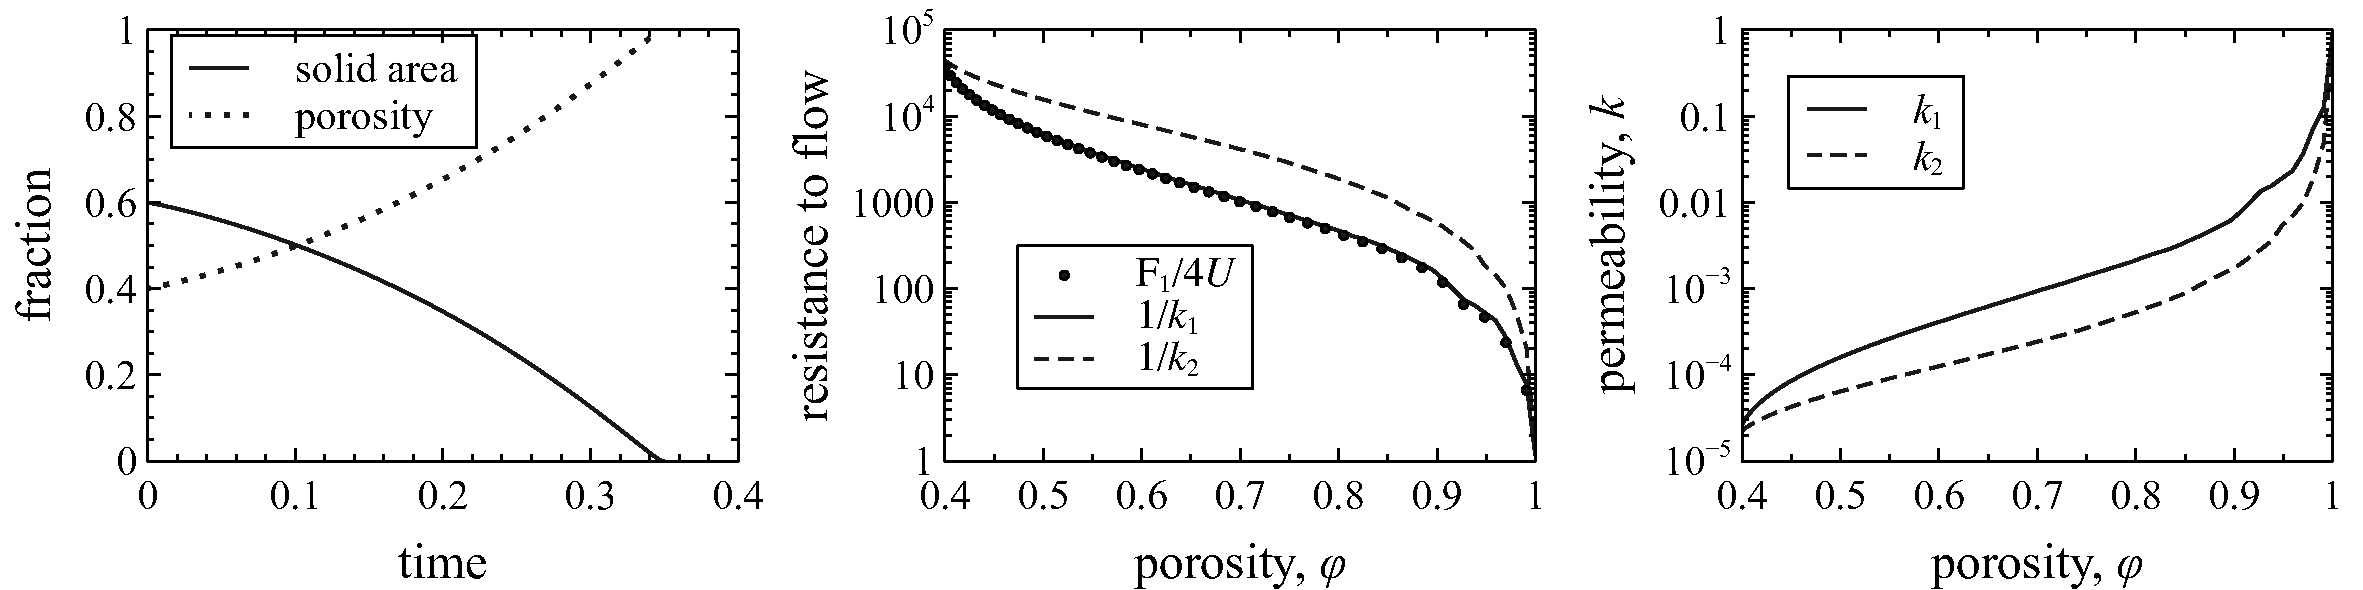
\includegraphics[width = 0.99 \textwidth]{./figs/fig2.pdf}
\caption{A single simulation of porous-medium erosion. The initial configuration consists of 100 circular bodies of random size and position, as seen in Fig.~1? a) As the medium erodes, the fraction of solid-body area decreases, or, equivalently, the porosity increases. b) Resistance to flow can be characterized by either the inverse permeability, $1/k$, or the cumulative drag, the two of which are related through \eqref{ResistDrag}. Both are seen to decrease as the medium erodes, and relationship \eqref{ResistDrag} is confirmed by the simulation data.
c) The relationship between permeability $k$ and porosity $\phi$ for the eroding medium. Both quantities increase with time as the medium erodes, but at different rates due to changes in the microstructure and channelization of the medium.
}
\end{figure*}
%---------------------------------------------------------%
% Data from 100-3


%---------------------------------------------------------%
\begin{figure*}%[htbp]
\centering \label{fig3}
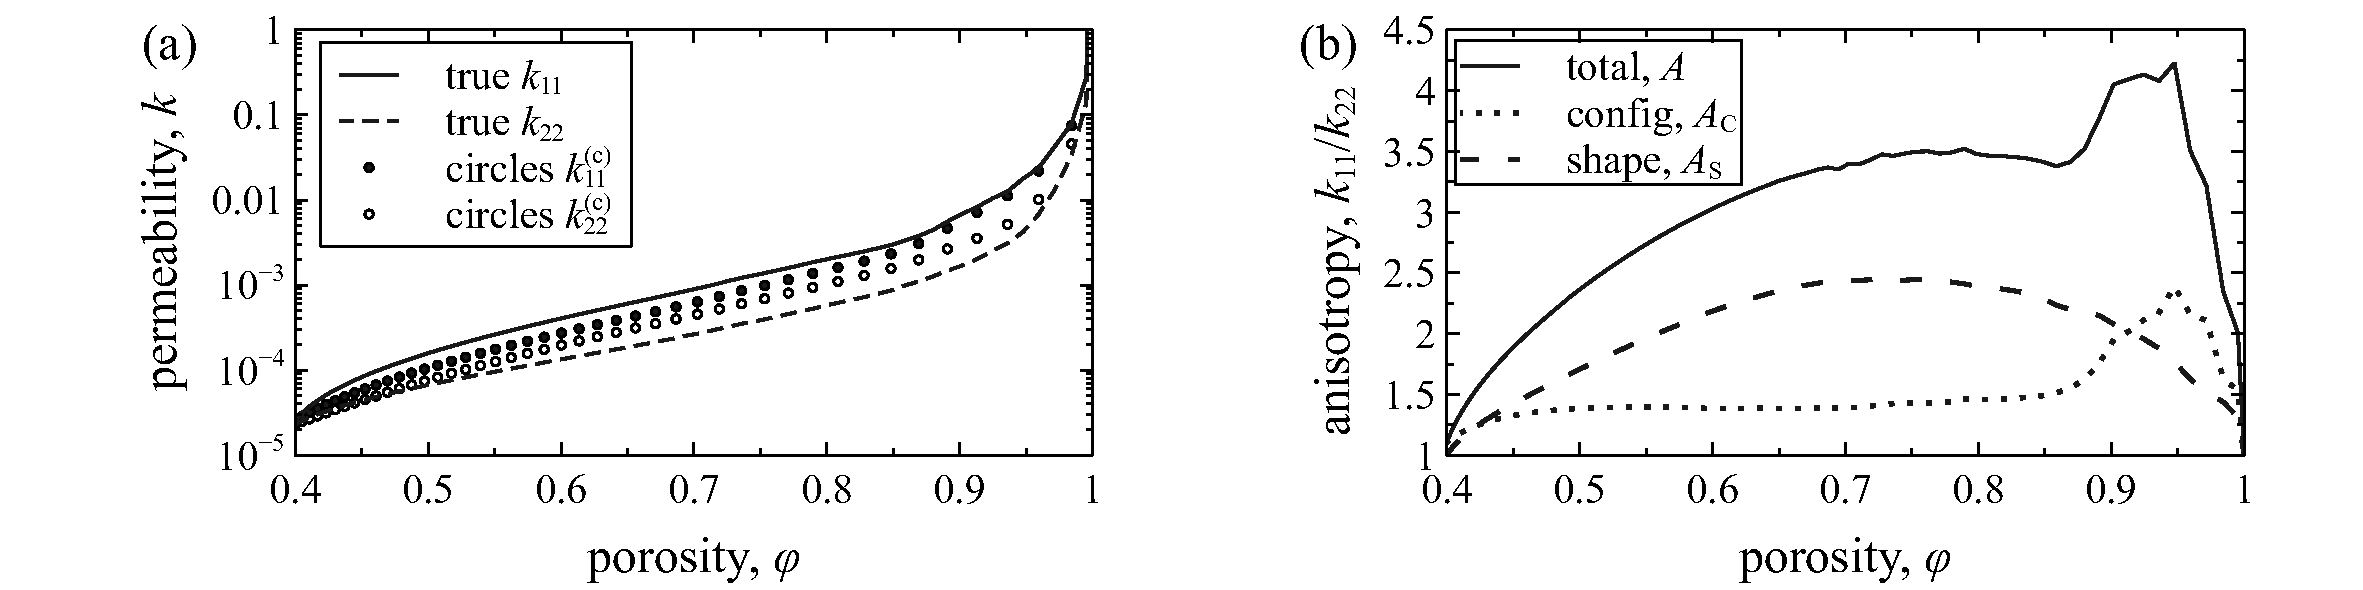
\includegraphics[width = 0.99 \textwidth]{./figs/fig3.pdf}
\caption{
Permeability
}
\end{figure*}
%---------------------------------------------------------%
% Data from 100-3


Text for Fig 3: 
The anisotropy of permeability grows large, up to a value of 4 during the middle portion of the simulation. The figure also shows the anisotropy of the circular grid.

%---------------------------------------------------------%
\begin{figure*}%[htbp]
\centering \label{fig4}
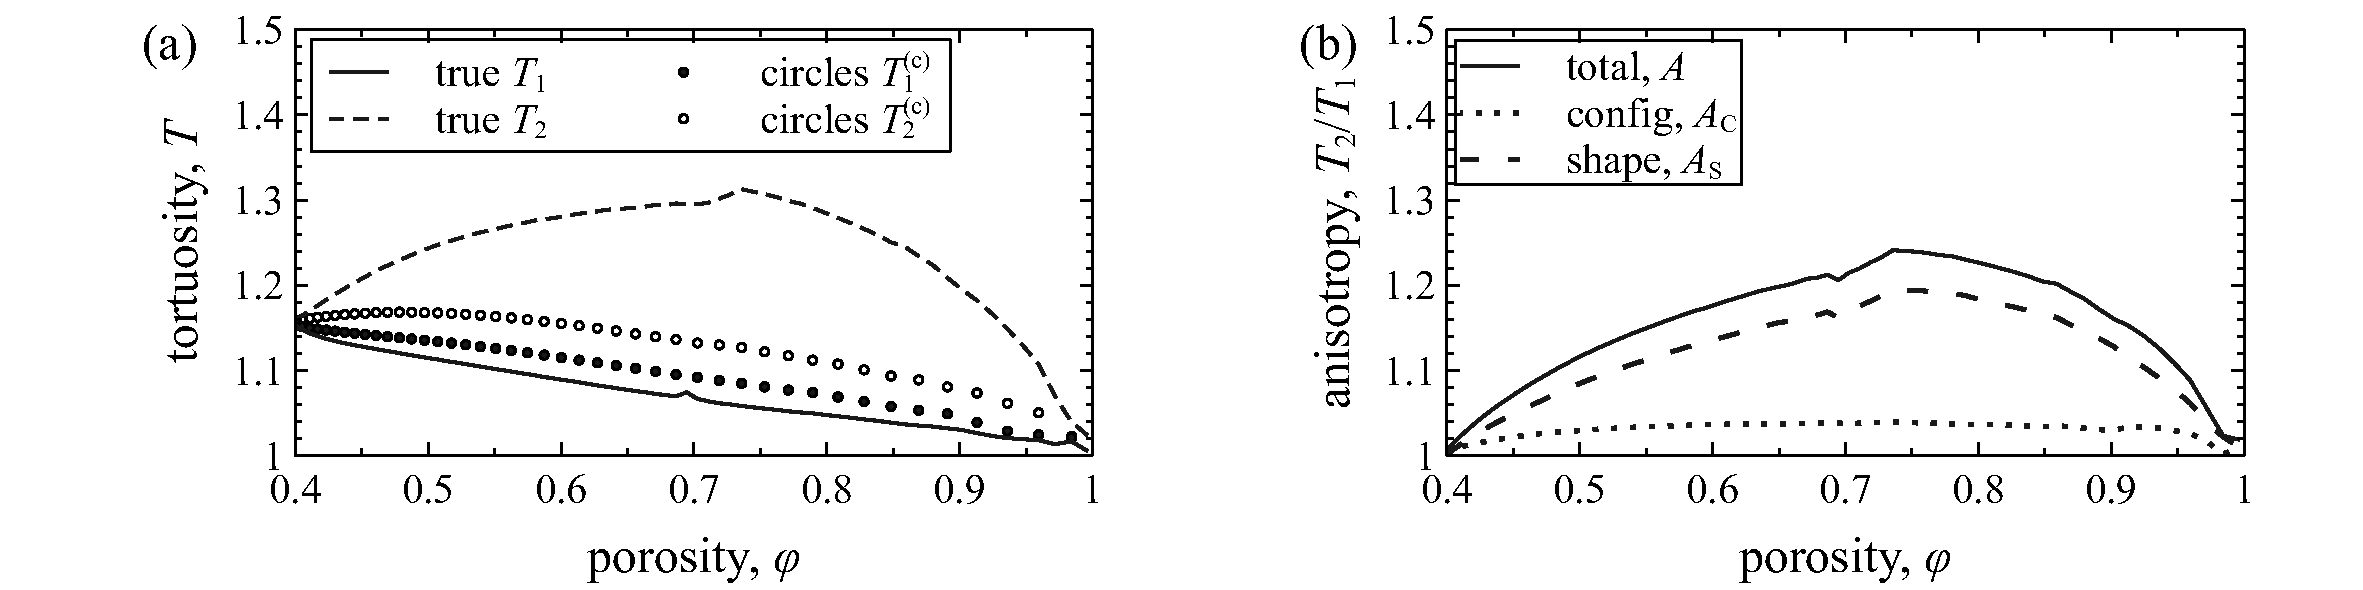
\includegraphics[width = 0.99 \textwidth]{./figs/fig4.pdf}
\caption{
Tortuosity
}
\end{figure*}
%---------------------------------------------------------%

%---------------------------------------------------------%
\begin{figure*}%[htbp]
\centering \label{fig5}
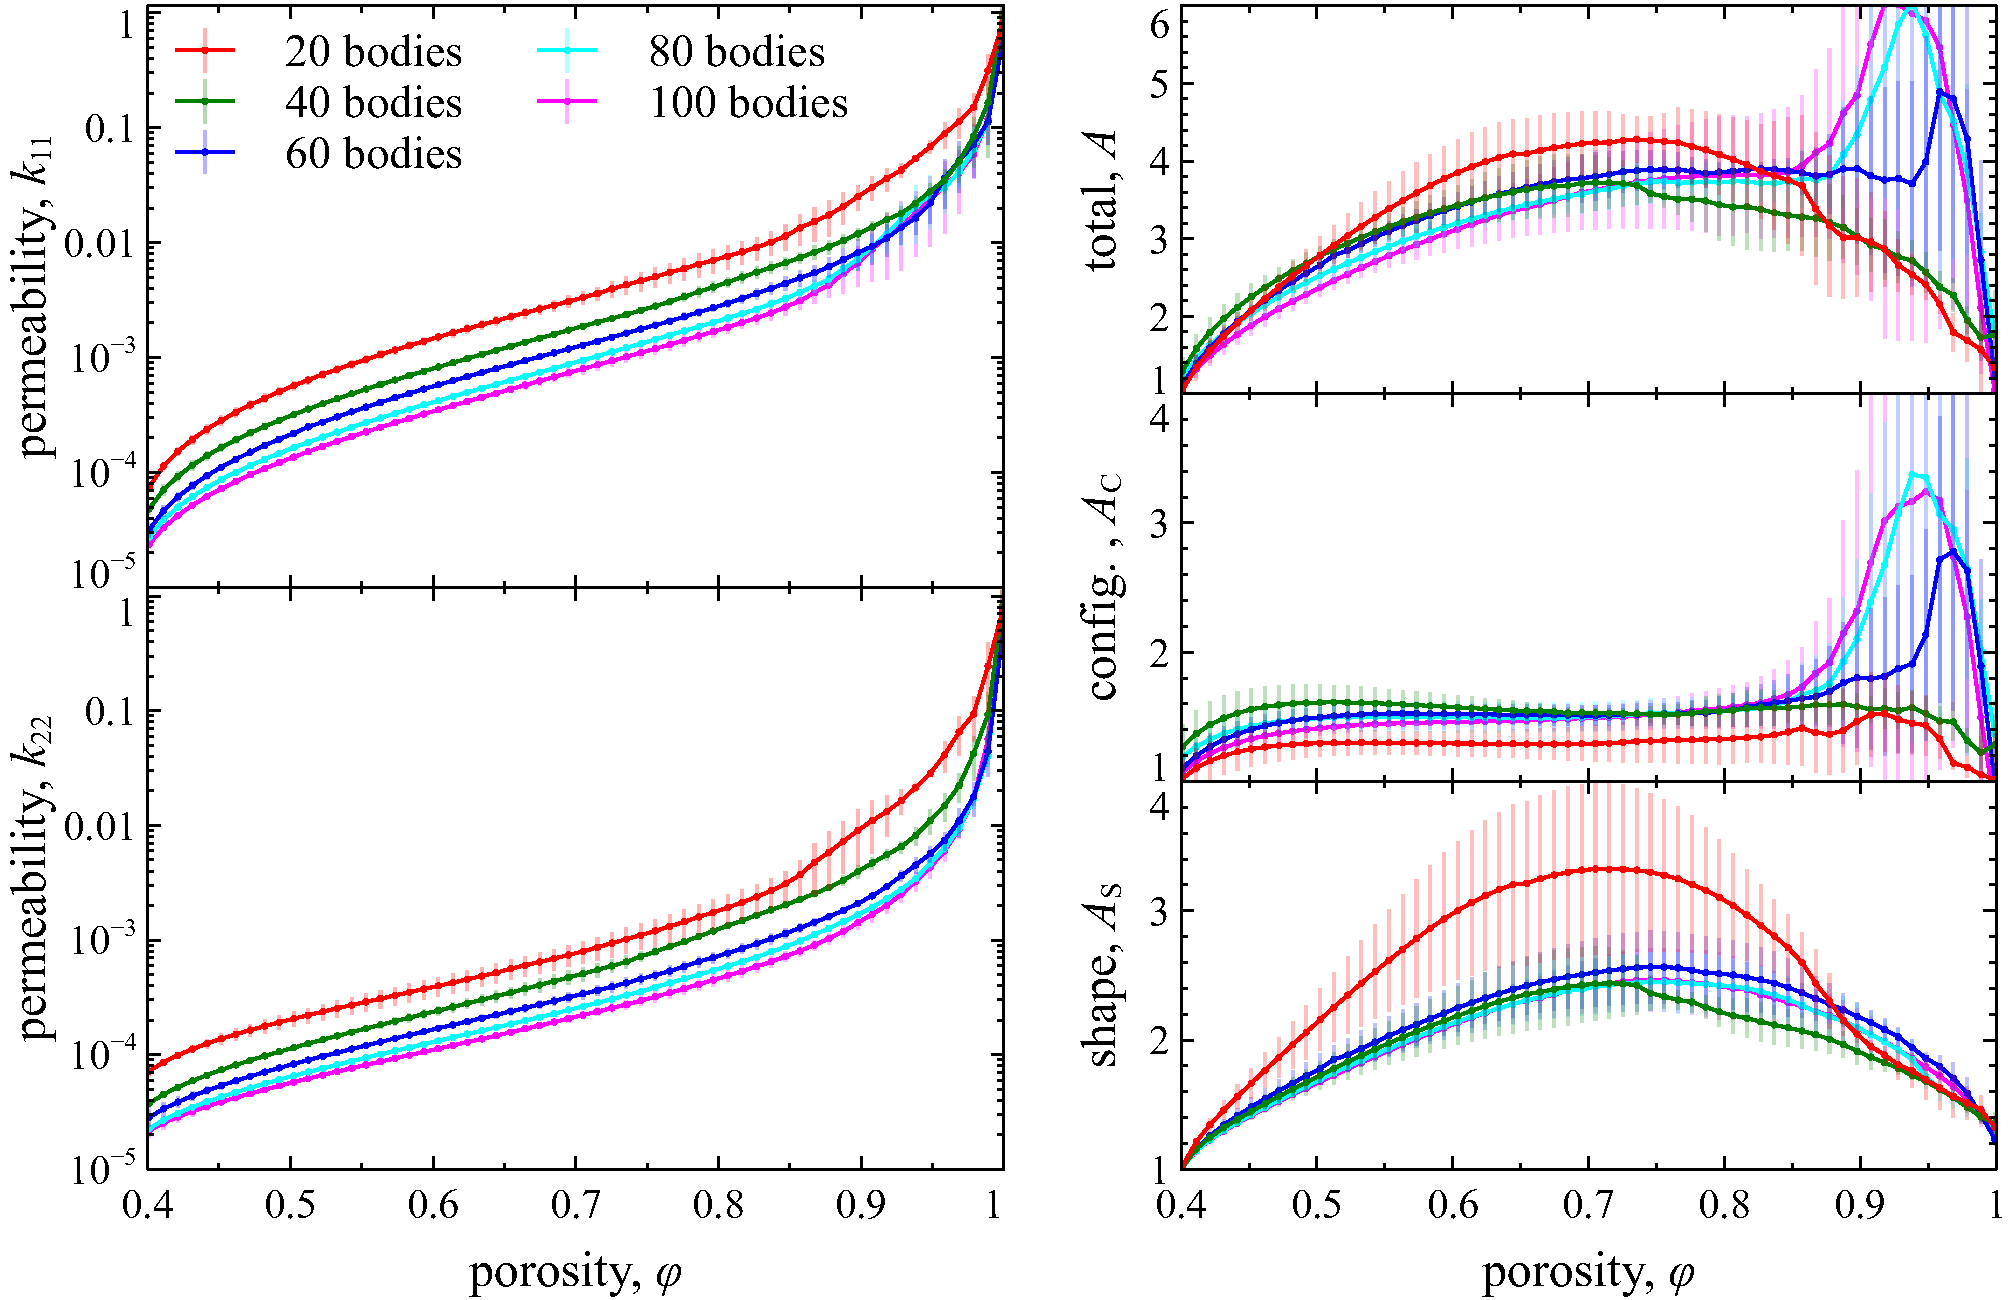
\includegraphics[width = 0.99 \textwidth]{./figs/fig5.pdf}
\caption{
a) Statistics from an ensemble of runs.
}
\end{figure*}
%---------------------------------------------------------%

%---------------------------------------------------------%
\begin{figure*}%[htbp]
\centering \label{fig6}
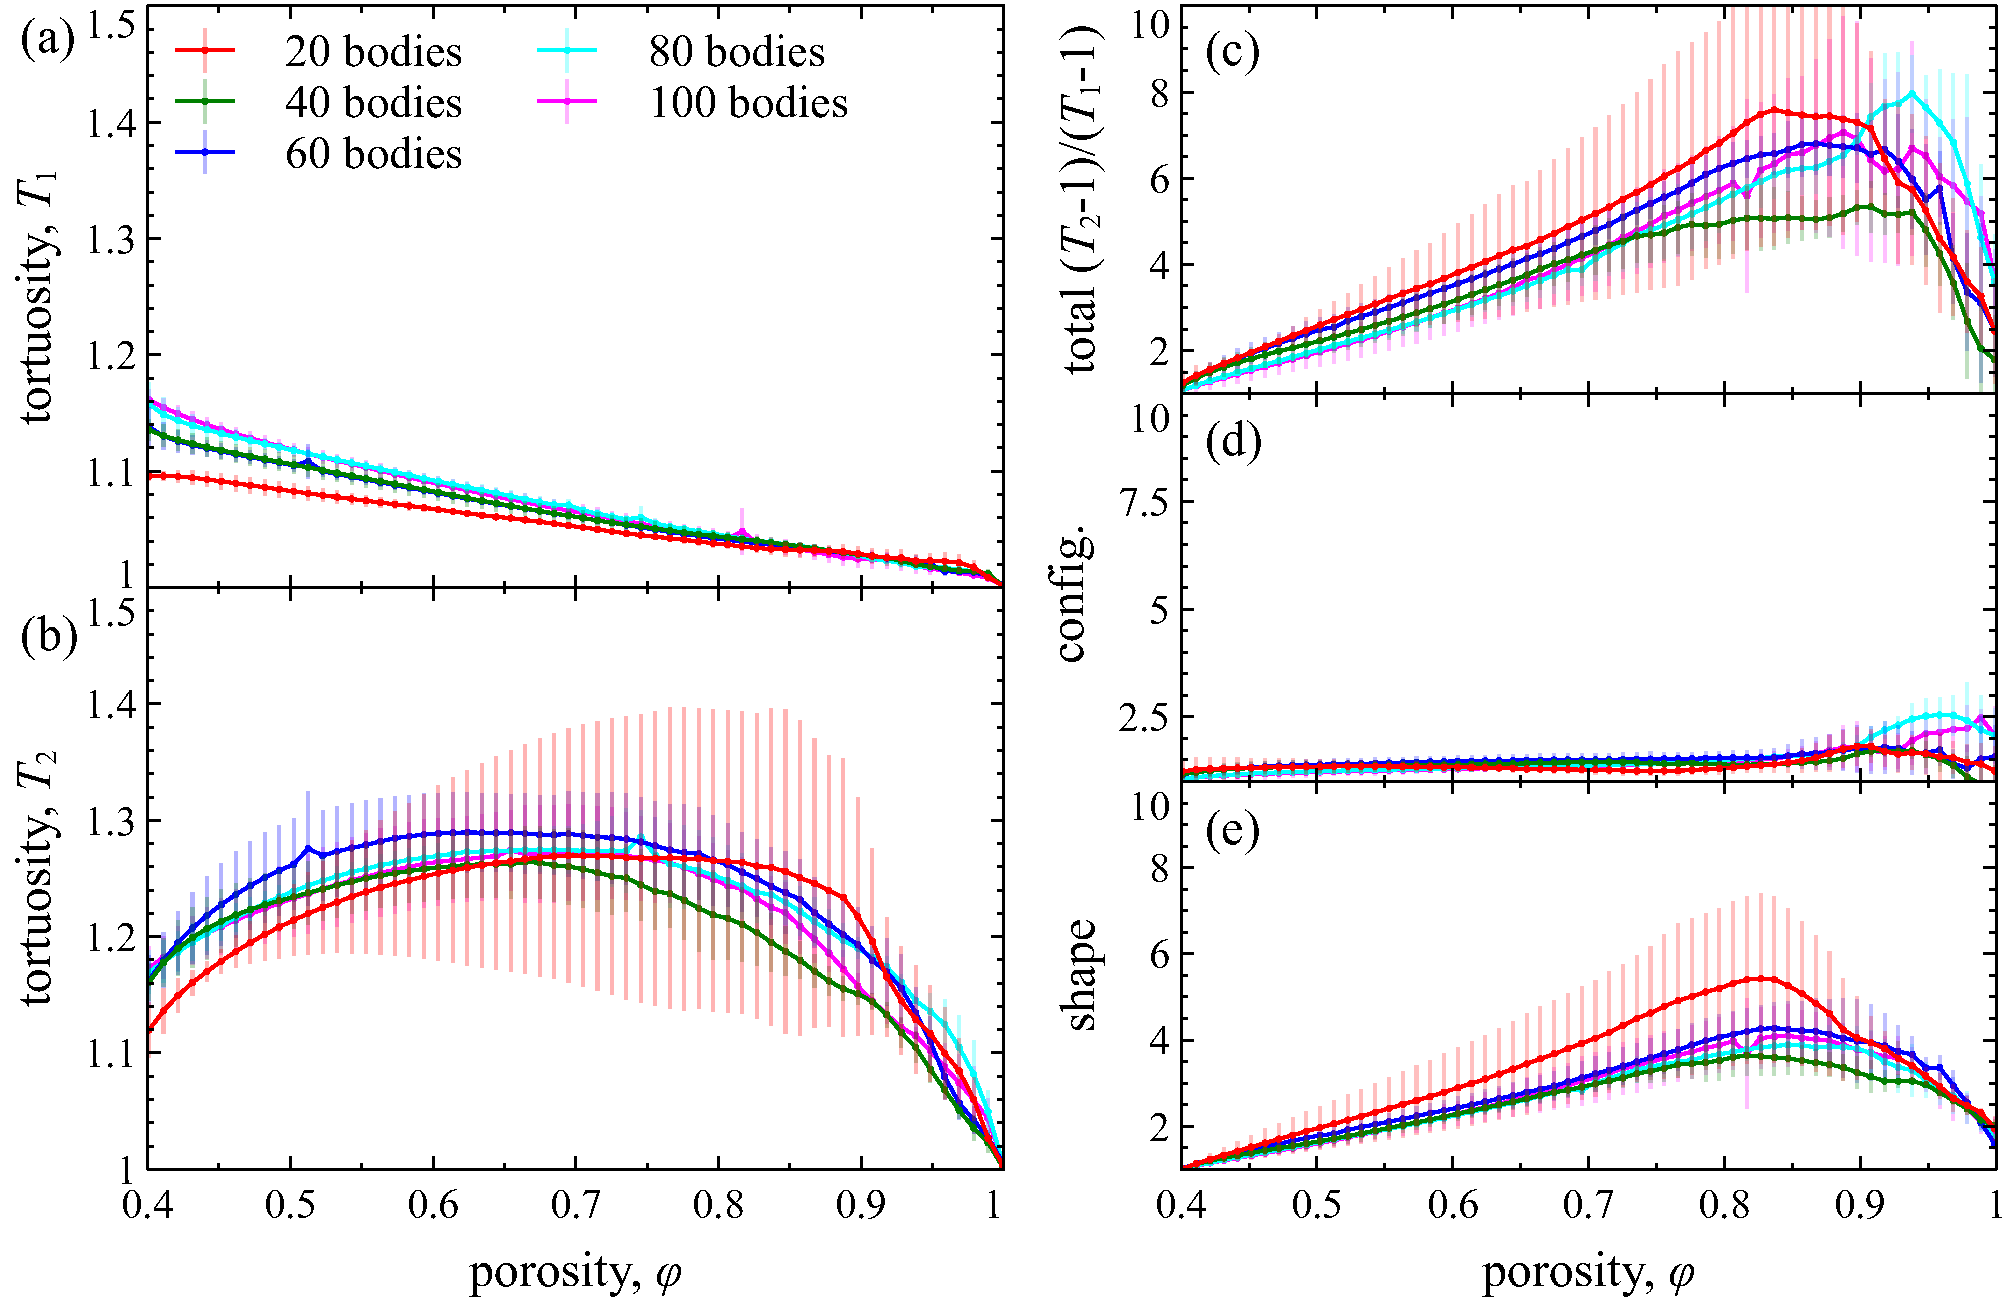
\includegraphics[width = 0.99 \textwidth]{./figs/fig6.pdf}
\caption{
a) Statistics from an ensemble of runs.
}
\end{figure*}
%---------------------------------------------------------%

\bibliographystyle{plain}
\bibliography{refs}
\end{document}
